\begin{figure}[htbp]
    \caption{Subsetting by contributor communication intensity}
    \label{fig}
    \centering
    \begin{minipage}[b]{0.49\textwidth}
        \centering
        \subcaption{Communication (lifetime)} \label{fig}
        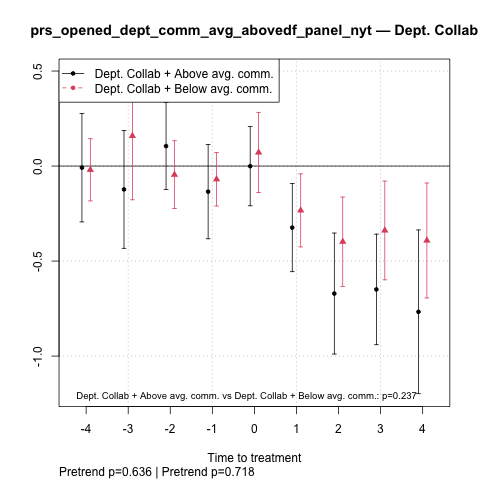
\includegraphics[width=\textwidth]{temp/output/collab/cs_norm_prs_opened_dept_comm_avg_above_Dept.Collab.png}
    \end{minipage}
    \hfill
    \begin{minipage}[b]{0.49\textwidth}
        \centering
        \subcaption{Communication per Problem}\label{fig}
        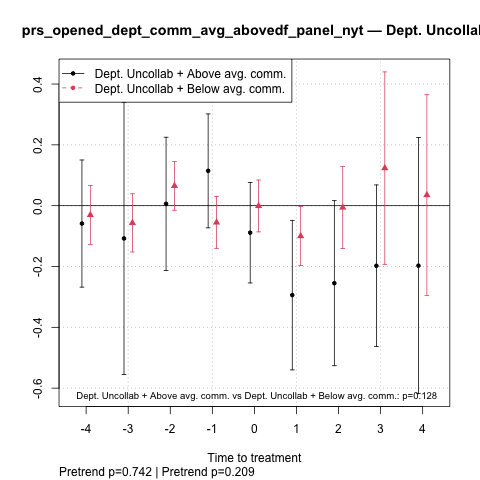
\includegraphics[width=\textwidth]{temp/output/collab/cs_norm_prs_opened_dept_comm_avg_above_Dept.Uncollab.png}
    \end{minipage}
        \begin{minipage}[b]{0.49\textwidth}
        \centering
        \subcaption{Communication (lifetime)} \label{fig}
        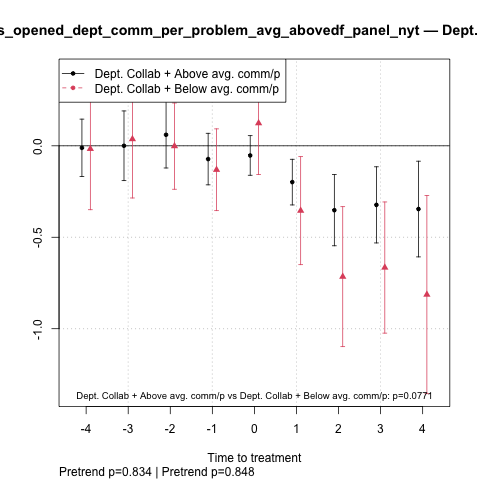
\includegraphics[width=\textwidth]{temp/output/collab/cs_norm_prs_opened_dept_comm_per_problem_avg_above_Dept.Collab.png}
    \end{minipage}
    \hfill
    \begin{minipage}[b]{0.49\textwidth}
        \centering
        \subcaption{Communication per Problem}\label{fig}
        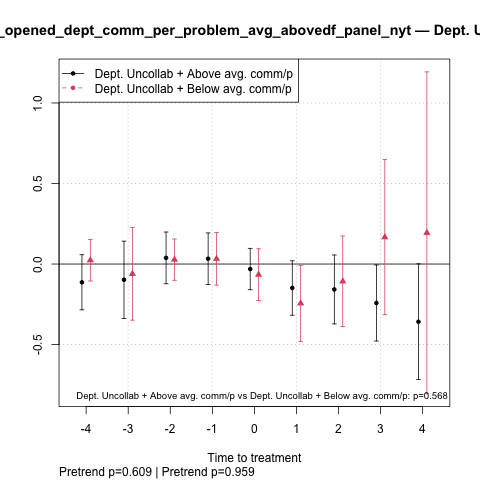
\includegraphics[width=\textwidth]{temp/output/collab/cs_norm_prs_opened_dept_comm_per_problem_avg_above_Dept.Uncollab.png}
    \end{minipage}


\todo[inline]{Graph improvements
1. Align axis for Panel a and b to -3.5 to 4.5 with ticks at every .5 (or 1)\\
2. Add figure notes describing definition of collaboration, confidence intervals (bootstrap 95 CI). \\
3. Change legend to indicate "Departed Contributor Collaborativeness" and have values be collaborative uncollaborative. \\
4. Remove grid background\\
5. Change time to treatment to "event time (k)"\\
6. Remove ugly bold label\\
7. Fine tune the plot subtitles
}

\end{figure}
